\documentclass[11pt]{article}

\usepackage{float}
\usepackage[a4paper, margin=2cm]{geometry}
\usepackage{graphicx}
\usepackage{setspace}

\chardef\_=`_

\title{\textbf{Trabalho Prático de Sistemas Operativos}}
\author{
    \begin{centering}
        \textbf{Grupo TPSO2}
    \end{centering} \\
    \begin{tabular}{ll}
        Humberto Gomes & A104448 \\
        José Lopes     & A104541 \\
        José Matos     & A100612
    \end{tabular}
}
\date{7 de maio de 2024}

\begin{document}

\onehalfspacing
\setlength{\parskip}{\baselineskip}
\setlength{\parindent}{0pt}
\def\arraystretch{1.5}

\maketitle

\begin{abstract}
    % TODO
\end{abstract}

\section{Arquitetura multiprocesso}

% TODO

\section{Arquitetura modular}

A arquitetura do \emph{software} desenvolvido pode ser abordada de diversas perspetivas, tal como a
da organização do código em diversos módulos, vistos na figura abaixo: \\

\begin{figure}[H]
    \centering
    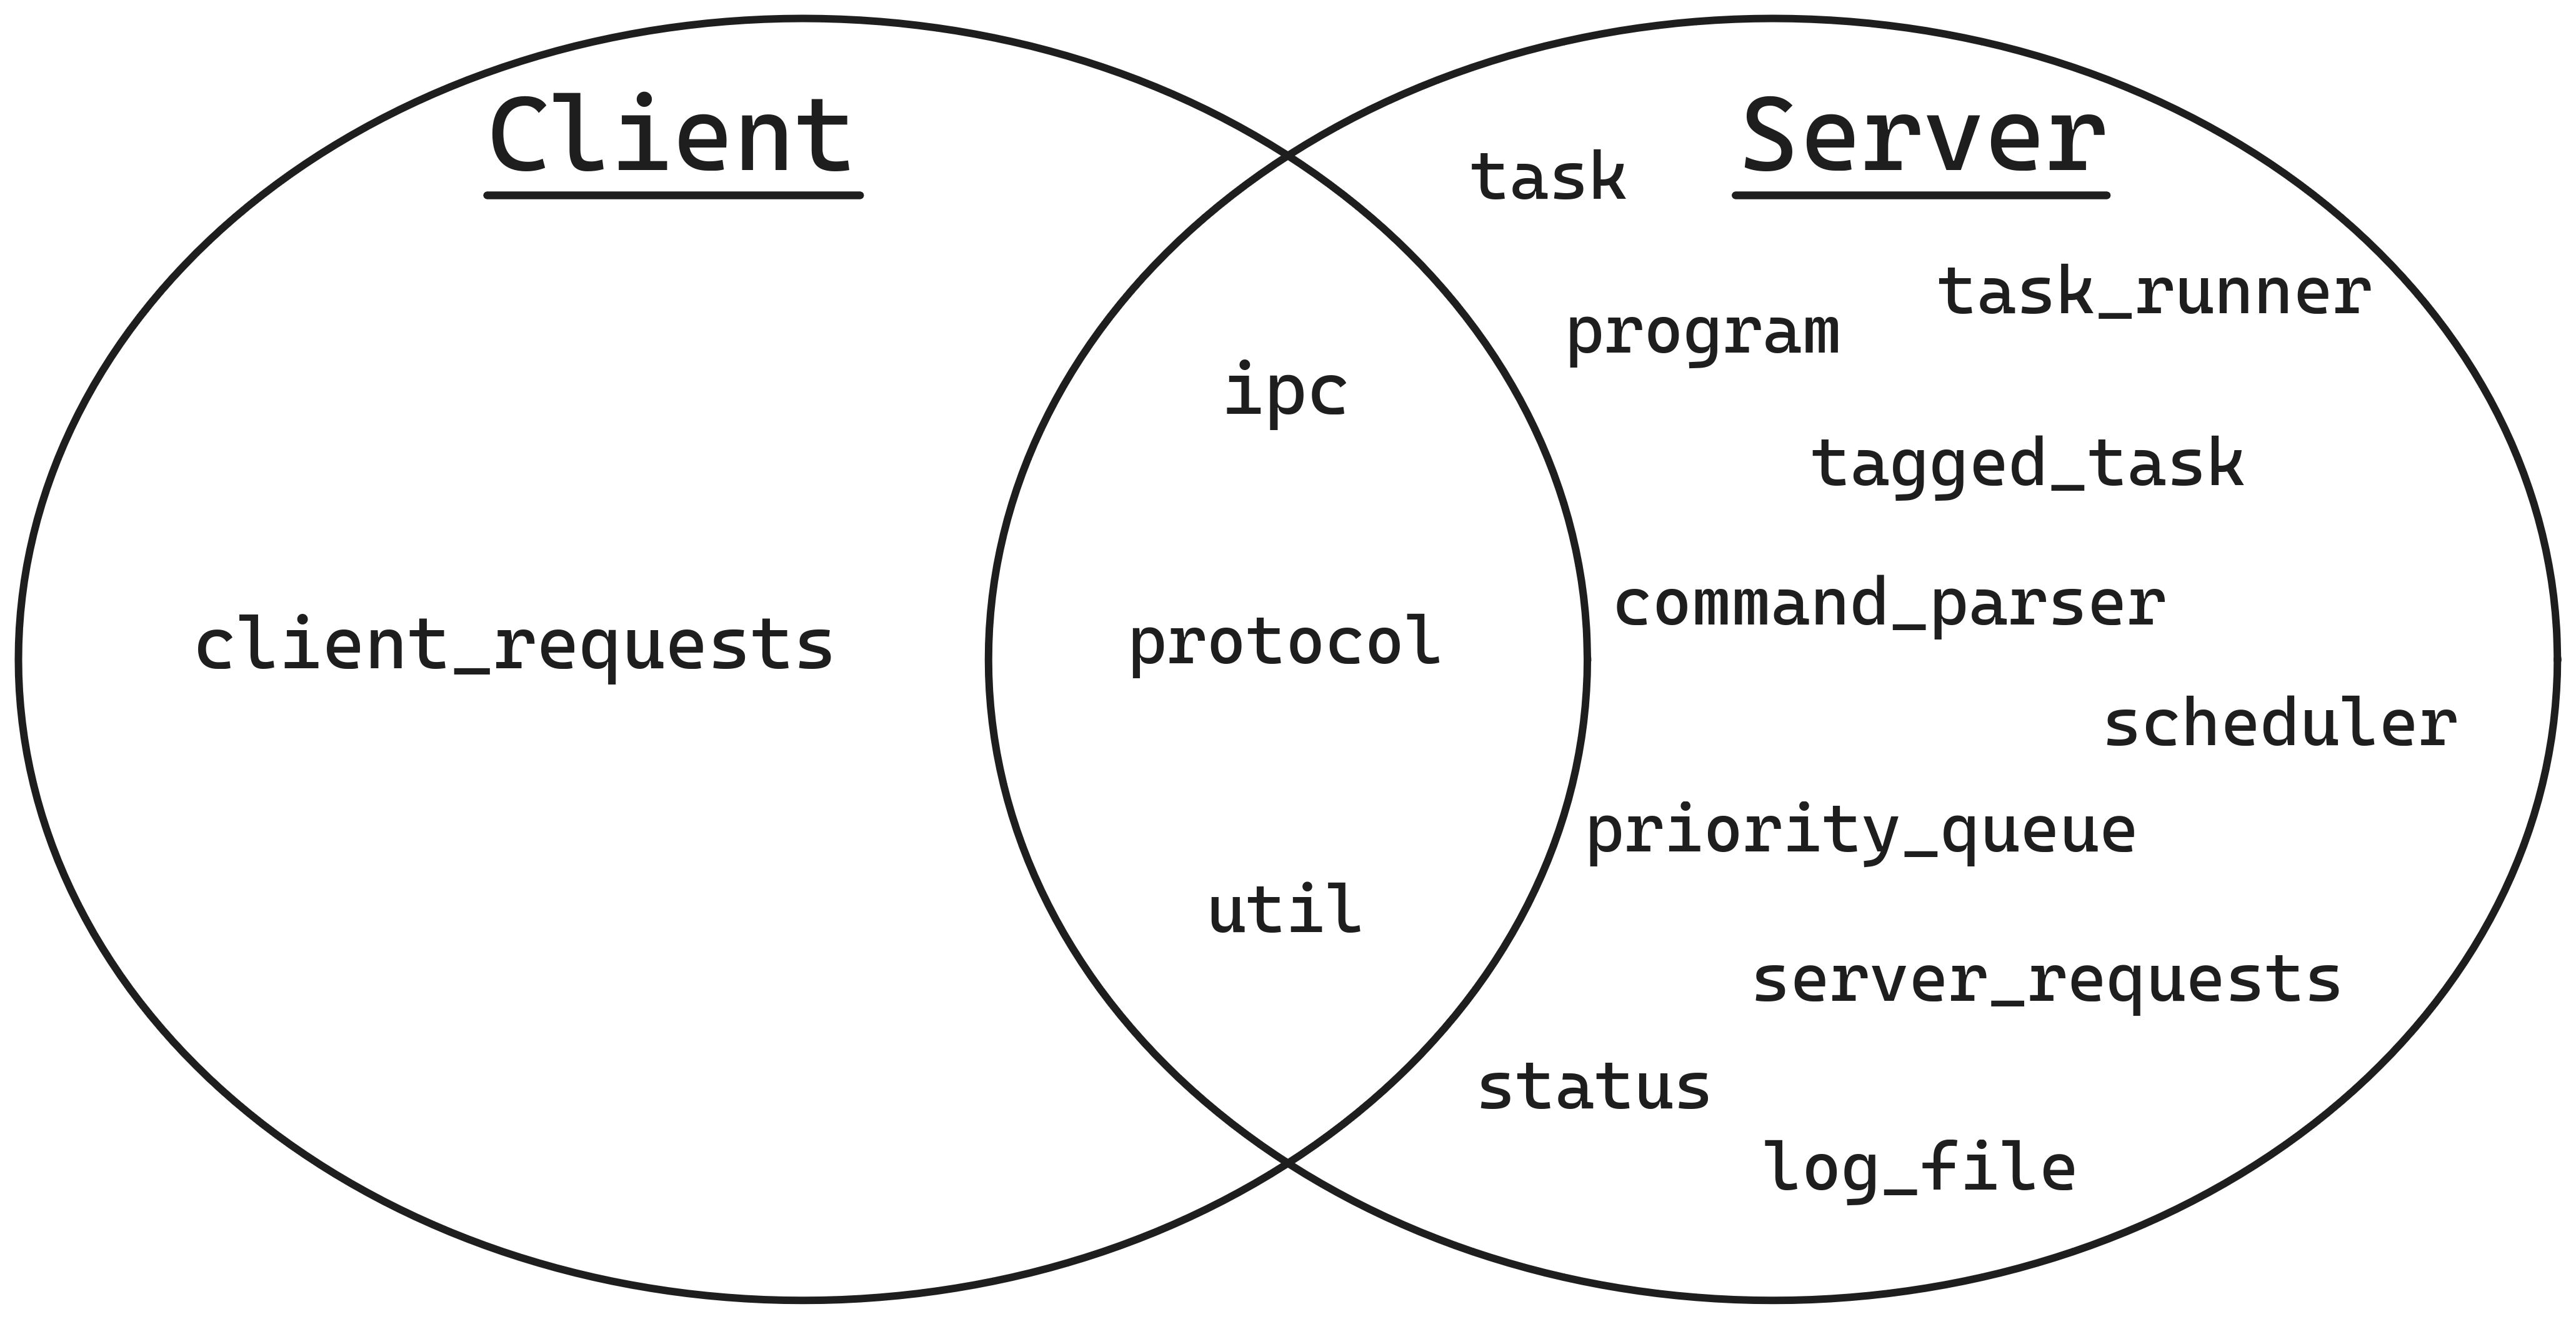
\includegraphics[width=0.6\textwidth]{report_figures/modules_venn_diagram.png}
    \caption{Módulos presentes no cliente e no servidor.}
\end{figure}

Alguns módulos são partilhados pelo cliente e pelo servidor: \texttt{util} fornece utilidades de
escrita para \texttt{stdout} e \texttt{stderr} utilizando a \emph{system call} \texttt{write};
\texttt{ipc} é responsável pela comunicação interprocesso a um nível mais básico (abertura de
conexões e separação de mensagens) utilizando \emph{pipes} com nome, enquanto que em
\texttt{protocol} estão definidas as estruturas das mensagens serializadas, transmitidas entre o
cliente e o servidor, e vice-versa.

O único módulo presente apenas no cliente é \texttt{client\_requests}, que é responsável por enviar
mensagens ao servidor e receber as suas respostas. No servidor, o módulo \texttt{server\_requests}
tem o papel dual: espera por pedidos do cliente para lhes responder. Este módulo é também
responsável por coordenar, conforme as mensagens que são recebidas, as escritas para o ficheiro de
\emph{logs}, feitas pelo módulo \texttt{log\_file}.

Há várias estruturas de dados no servidor. \texttt{program} é um \emph{array} de argumentos
terminado em \texttt{NULL}, facilmente providenciado a uma função na família \texttt{exec}. Vários
programas formam uma \emph{pipeline} em \texttt{task}, que alternativamente pode ser constituída por
um procedimento de C (é possível escalonar tarefas que não programas independentes). Há mais
informação necessária para a gestão de tarefas do que uma lista de programas, como identificadores e
tempos em filas de espera. Uma \texttt{tagged\_task} é formada por uma \texttt{task} e por esta
informação. Continuando-se a cadeia de composição, tem-se a estrutura \texttt{priority\_queue}, uma
\emph{minheap} de tarefas, onde definir uma política de escalonamento se torna tão simples como
definir uma função de comparação entre tarefas.

Vários outros módulos são responsáveis pela funcionalidade do servidor. Apesar de uma \texttt{task}
poder ser criada manualmente, programa a programa, a funcionalidade de interpretação de uma
\emph{string} de linha de comandos é providenciada pelo módulo \texttt{command\_parser}.
\texttt{scheduler} é responsável por saber que tarefas estão em execução e em fila de espera,
criando novos processos para a execução de novas tarefas desde que tenha disponibilidade para tal.
Há dois programas que são executados, \texttt{status}, responsável por enviar ao cliente informação
sobre o servidor sem o bloquear, e \texttt{task\_runner}, responsável pela execução de tarefas
como \emph{pipelines}, informando o processo pai do orquestrador quando estas terminam.

A arquitetura modular utilizada foi essencial para o \emph{software} desenvolvido. Não só garante
código de melhor qualidade, como permite evitar erros (como erros de memória e invariantes violadas)
que ocorrem devido à quebra do encapsulamento. A manutenção do código também se tornou mais simples.
Por exemplo, foi necessária, devido a um \emph{bug} que não se conseguiu resolver, a mudança
completa do protocolo definido em \texttt{ipc.c}. Foi possível reescrever este ficheiro mantendo a
interface das funções nele definidas, e o servidor manteve-se operacional sem qualquer outra mudança
necessária.

\section{Testes executados}

Foram escritos testes para avaliar diversos aspetos do \emph{software} desenvolvido, tanto de um
ponto de vista funcional como de desempenho. Nesta secção são descritos os testes desenvolvidos e
as correções que deles resultaram.

O teste \texttt{fds.sh} verifica quais são os descritores de ficheiro abertos num processo criado
pelo servidor em qualquer posição possível numa \emph{pipeline}. Em princípio, o descritor 0
(\texttt{stdin}) devia estar aberto para todos os processos que não o primeiro da \emph{pipeline}, e
os descritores 1 e 2 (\texttt{stdout} e \texttt{stderr}) deveriam ser os únicos restantes abertos.
No entanto, outros descritores abertos foram detetados e o código de \texttt{task\_runner} foi
corrigido para fechar alguns descritores de \emph{pipes} que se mantinham abertos. Este é o único
teste que não corre em outros sistemas POSIX que não Linux, pois precisa de acesso à diretoria
\texttt{/proc/self/fd}.

De seguida, o teste \texttt{length.sh} verifica que o servidor suporta corretamente mensagens com o
comprimento máximo especificado. Inicialmente, tarefas com comandos muito longos podiam ser
escalonadas, mas não surgiam num pedido de \texttt{status} do cliente. São necessários limites de
comprimento para garantir a atomicidade de escritas no FIFO. Caso o comprimento do comando de uma
tarefa seja superior ao permitido por uma mensagem de estado, o comando é substituído pela
\emph{string} \texttt{"COMMAND TOO LONG"}.

O teste \texttt{order.sh} garante que os processos enviados ao servidor são escalonados corretamente
conforme a política de escalonamento definida. Este teste não revelou qualquer erro no comportamento
do servidor. Outro teste que não revelou problemas foi \texttt{parser.sh}, que garante que o
\emph{parser} de linhas de comando funciona como esperado. Outro teste que não exigiu alterações ao
código escrito foi \texttt{pipelines.sh}, que testa se os processos de uma tarefa são executados
corretamente, permitindo que os \emph{pipes} entre eles transmitam mais informação do que a sua
capacidade. Fá-lo através da transferência de um vídeo do YouTube, aplicando efeitos ao seu áudio, e
reproduzindo-o, sem alguma vez escrever para o sistema de ficheiros.

Ademais, o teste \texttt{status.sh} procura verificar se o servidor consegue enviar o seu estado ao
cliente corretamente. Detetou-se perda de mensagens quando em elevadíssimo número, erro cuja causa
não se conseguiu descobrir, levando a que o módulo \texttt{ipc} fosse reescrito para deixar de usar
mensagens de comprimento variável, passando a utilizar mensagens de comprimento fixo.

De seguida, \texttt{stress.sh} cria milhares de processos de clientes, que tentam comunicar com o
servidor em simultâneo pelo FIFO partilhado. Detetou-se a possibilidade do servidor fechar o seu
descritor durante a escrita de um cliente, resultando na terminação deste com um \texttt{SIGPIPE}.
Não é um grande problema o cliente falhar, mas esta falha de comunicação pode ocorrer quando um
processo filho do orquestrador tenta avisar o seu pai que a sua execução está prestes a terminar.
Se o servidor não receber esta mensagem, nunca saberá que um dos seus filhos terminou e que passa a
ter mais capacidade de escalonamento disponível. Foi-nos permitido pelo regente da UC ignorar o
sinal através da \emph{system call} \texttt{signal}, permitindo que \texttt{write} termine com um
código de erro, podendo retentar-se a comunicação com o servidor.

Por último, o ficheiro \texttt{benchmark.sh} procura analisar o desempenho do servidor, fazendo
pedidos de cem tarefas de duração entre 300 milissegundos e 2 segundos, executado para as políticas
de escalonamento FCFS e SJF. No final, o estado do servidor é requisitado, revelando informação
sobre o tempo de espera e de execução das tarefas, que sofre uma conversão para um formato CSV,
importado para uma folha de cálculo e analisado:

\begin{figure}[H]
    \centering
    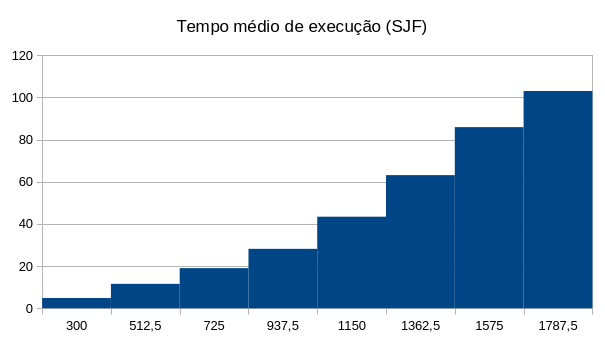
\includegraphics[width=0.45\textwidth]{report_figures/HistogramSJF.png}
    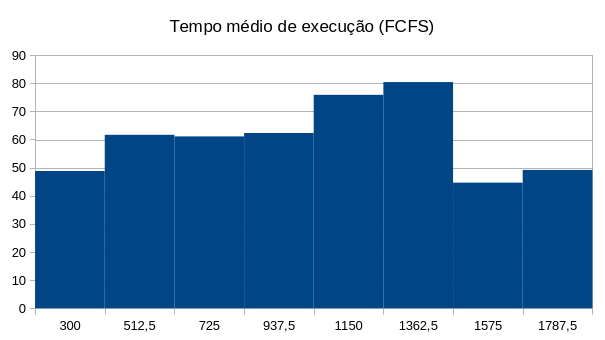
\includegraphics[width=0.45\textwidth]{report_figures/HistogramFCFS.png}
    \caption{Tempos médios de execução de tarefas (desde o cliente até o fim da execução, em
        segundos) em função da sua duração (em milissegundos), agrupada em oito conjuntos, conforme
        a política de escalonamento usada.}
\end{figure}

\begin{figure}[H]
    \centering
    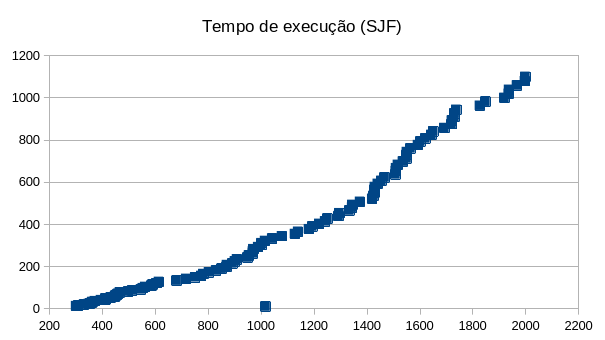
\includegraphics[width=0.45\textwidth]{report_figures/ScatterSJF.png}
    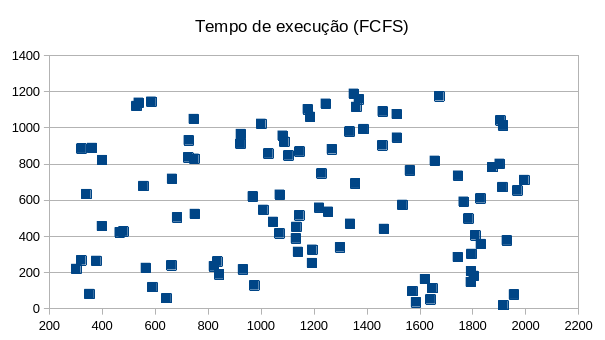
\includegraphics[width=0.45\textwidth]{report_figures/ScatterFCFS.png}
    \caption{Tempos de execução de tarefas (desde o cliente até o fim da execução, em segundos) em
        função da sua duração (em milissegundos), conforme a política de escalonamento usada.}
\end{figure}

Conforme esperado, quando a política \emph{Shortest Job First} é utilizada, tarefas de menor duração
passam menos tempo em fila de espera (a maior contribuição para o tempo total de execução) do que as
tarefas mais longas, evidenciado pelo comportamento linear tanto no histograma como no
\emph{scatter}. Por outro lado, o tempo de execução quando se aplica a política \emph{First Come
First Served} é relativamente uniforme, evidenciado pela altura relativamente próxima das barras do
histograma e da aleatoriedade no \emph{scatter}.

Como na política SJF as tarefas mais rápidas são executadas em primeiro lugar, os tempos de espera
das primeiras tarefas são muito baixos, reduzindo o tempo médio de espera total. Esta tese
verifica-se: SFJ apresenta um tempo médio de espera de 402 segundos mas estes tornam-se 592 segundos
para FCFS. No entanto, em FCFS, tarefas de maior duração experienciam menor tempo médio, como se
observa no primeiro par de gráficos. Logo, a escolha de uma política de escalonamento depende do
tipo de tarefa que se pretende valorizar: usa-se SJF para processos de menor duração e FCFS para
tarefas mais longas.

\section{Decisões relevantes}

Nesta secção, são discutidas algumas decisões tomadas ao longo do desenvolvimento do projeto, que
julgamos serem relevantes de mencionar.

Inicialmente, o nosso grupo pensava em fazer um orquestrador seguro, capaz de estar presente num
sistema partilhado (\emph{multiseat}). No entanto, foi rápida a conclusão de que sem virtualização
(ou \emph{containerização}) seria possível um cliente enviar uma tarefa como \texttt{pkill
orchestrator}. Ademais, poderiam ser envidas várias tarefas sem fim, tirando toda a capacidade ao
servidor, sem que este as possa matar devido à impossibilidade de se utilizarem sinais. Logo, o
objetivo de segurança foi descartado e o nosso foco passou para a robustez do servidor, que foi
programado de modo a resistir a erros tanto internos (como \emph{system calls} falhadas) como
externos (mensagens mal formatadas no FIFO), procurando recuperar e voltar a um estado conhecido.
Ademais, durante o desenvolvimento era executado o \texttt{valgrind}, para procurar erros de memória
como acessos indevidos à memória e \emph{memory leaks}. Após os vários testes realizados e falhas
propositadamente provocadas, julgamos que o servidor seja capaz de continuar a operar corretamente
sem \emph{crashes}.

De seguida, optámos por utilizar uma \emph{minheap} (\texttt{priority\_queue}) para as políticas de
escalonamento SJF e FCFS, apesar de tal não conduzir ao melhor desempenho. \emph{Minheaps}
apresentam complexidades (caso médio) de $\Theta(1)$ para inserção e $\Theta(\log n)$ para remoção.
Estas são ideais para SJF, mas seria possível uma remoção em tempo constante para FCFS caso se
utilizasse uma fila simples. No entanto, por motivos de simplicidade, preferiu-se o uso de uma única
estrutura de dados com pior desempenho do que a adição de código necessária para se suportarem duas
estruturas.

Por último, julgamos importante mencionar que fomos contra a recomendação do enunciado de utilizar a
\emph{system call} \texttt{gettimeofday} para a medição de intervalos temporais, utilizando
\texttt{clock\_gettime} no seu lugar. \texttt{gettimeofday} é uma função depreciada desde 2008,
sendo que a sua substitução, \texttt{clock\_gettime}, já foi introduzida em 2001, pelo que o seu uso
não afetaria a portabilidade do \emph{software} desenvolvido. Ademais, esta função, quando usada com
\texttt{CLOCK\_MONOTONIC}, não é influenciada por mudanças no relógio do computador (por exemplo,
um ajuste do utilizador), garantindo sempre que o valor de tempo devolvido aumenta e que não se
calculam intervalos de tempo negativos.

\section{Conclusão}

% TODO

\end{document}
